\subsection{Basic calculations}
\subsubsection{Addition / subtraction}
$(\mathbf {A}+\mathbf {B})_{i,j}=\mathbf {A}_{i,j}+{\mathbf {B}}_{i,j},\quad 1\leq i\leq m,\quad 1\leq j\leq n$\\
$(\mathbf {A}-\mathbf {B})_{i,j}=\mathbf {A}_{i,j}-{\mathbf {B}}_{i,j},\quad 1\leq i\leq m,\quad 1\leq j\leq n$
\subsubsection{Scalar multiplication}
$(c\mathbf{A})_{i,j}=c\cdot A_{i,j}$
\subsubsection{Matrix multiplication}
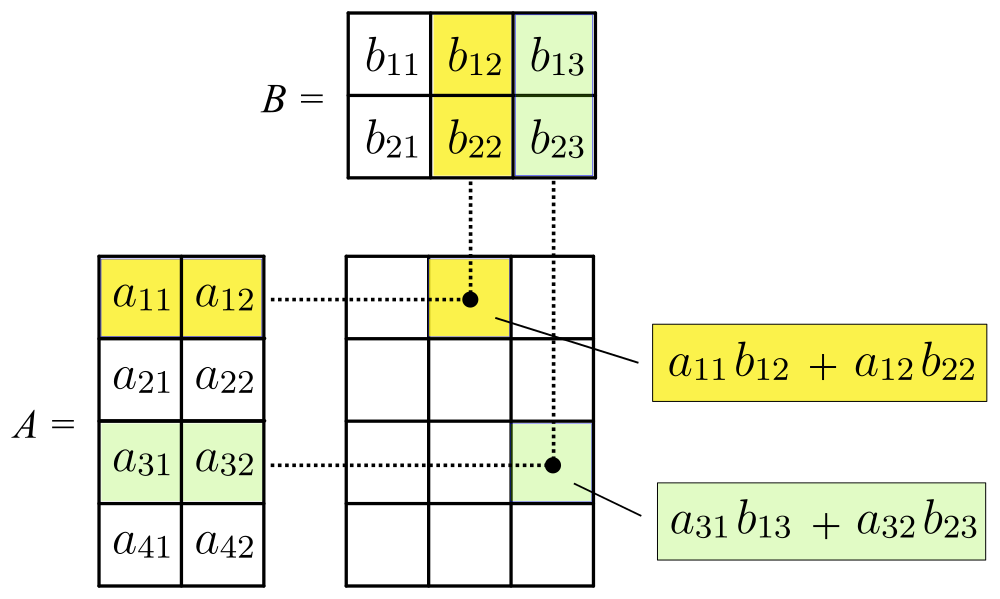
\includegraphics[width=0.35\textwidth]{MatrixMultiplication}

\subsubsection{Transposition}
$(\mathbf{A}^\mathrm{T})_{i,j}=A_{j,i}$

\subsection{Special matrices}
\begin{description}
	\item[Square matrix:] The number of rows and columns are the same
	\item[Zero matrix:] All of the elements are zero
	\item[Identity matrix:] A square matrix in which all the elements on the leading diagonal are 1 and the remaining elements are 0, denoted by $\mathbf{I}_k$ for $k\times k$ identity matrix
\end{description}


\subsection{Determinants}

\subsubsection{$2\times2$ matrices}
$\begin{vmatrix}a&b\\c&d\end{vmatrix}=ad-bc$

\subsubsection{$3\times3$ matrices}

$\begin{vmatrix}a&b&c\\d&e&f\\g&h&i\end{vmatrix}=a\begin{vmatrix}e&f\\h&i\end{vmatrix}-b\begin{vmatrix}d&f\\g&i\end{vmatrix}+c\begin{vmatrix}d&e\\g&h\end{vmatrix}=aei+bfg+cdh-ceg-bdi-afh$

\subsubsection{Singular matrices}
\begin{itemize}
	\item Singular matrices are square matrices with a determinant of 0
	\item It does not have an inverse
	\item If $\mathbf{A}$ and $\mathbf{B}$ are non-singular matrices, then $(\mathbf{AB})^{-1}=\mathbf{B}^{-1}\mathbf{A}^{-1}$
\end{itemize}



\subsubsection{Properties of determinants}
\begin{itemize}
	\item $\det(\mathbf{AB})=\det(\mathbf{A})\det(\mathbf{B})=\det(\mathbf{B})\det(\mathbf{A})=\det(\mathbf{BA})$
	\item $\det(k\mathbf{A})=k^n\det(\mathbf{A})$ ($\mathbf{A}$ is a $n\times n$ matrix)
\end{itemize}


\subsection{Inverse matrices}
\subsubsection{$2\times2$ matrices}
$\begin{bmatrix}
	a & b\\c & d
\end{bmatrix}^{-1}=\dfrac{1}{ad-bc}\begin{bmatrix}
	d & -b\\-c & a
\end{bmatrix}$

\subsubsection{$3\times3$ matrices}
$\mathbf {A} ^{-1}={\begin{bmatrix}a&b&c\\d&e&f\\g&h&i\\\end{bmatrix}}^{-1}={\frac {1}{\det(\mathbf {A} )}}{\begin{bmatrix}\,A&\,B&\,C\\\,D&\,E&\,F\\\,G&\,H&\,I\\\end{bmatrix}}^{\mathrm {T} }={\frac {1}{\det(\mathbf {A} )}}{\begin{bmatrix}\,A&\,D&\,G\\\,B&\,E&\,H\\\,C&\,F&\,I\\\end{bmatrix}}$\\
$\begin{alignedat}{6}A&={}&(ei-fh),&\quad &D&={}&-(bi-ch),&\quad &G&={}&(bf-ce),\\B&={}&-(di-fg),&\quad &E&={}&(ai-cg),&\quad &H&={}&-(af-cd),\\C&={}&(dh-eg),&\quad &F&={}&-(ah-bg),&\quad &I&={}&(ae-bd).\\\end{alignedat}$

\subsubsection{Solving equations with matrices}
If $\mathbf{A}\begin{pmatrix}
	x\\y\\z
\end{pmatrix}=\mathbf{v}$ then $\begin{pmatrix}
	x\\y\\z
\end{pmatrix}=\mathbf{A}^{-1}\mathbf{v}$
\begin{description}
	\item[Consistent system of linear equations:] there is at least one set of values that satisfies all the equations simultaneously
	\item[Inconsistent:] such set of values does not exist
\end{description}

\subsubsection{Possible outcomes of solutions}
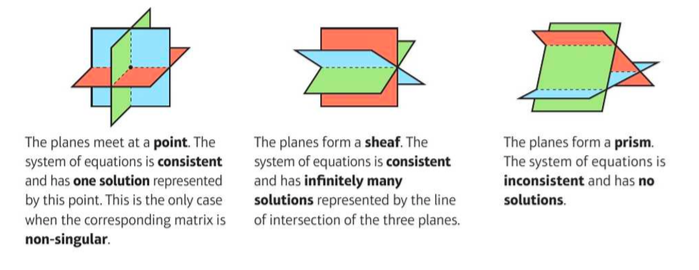
\includegraphics[width=0.75\textwidth]{equations}\\
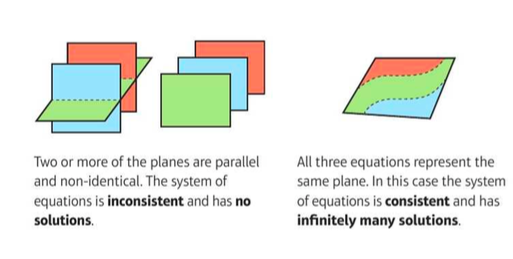
\includegraphics[width=0.5\textwidth]{equations2}

\subsection{Linear transformations}
\subsubsection{Properties}
If $L(\vec{v})$ is linear:
\begin{enumerate}
	\item $L(\vec{v})$ should always map the origin onto itself
	\item $L(\vec{v})$ can be represented by a matrix
	\item $L(\vec{v_1}+\vec{v_2})=L(\vec{v_1})+L(\vec{v_2})$ (closure in addition)
	\item $L(\lambda\vec{v_1})=\lambda L(\vec{v_1})$ (closure in scalar multiplication)
\end{enumerate}
\subsubsection{Invariant points and lines}
\begin{description}
	\item[Invariant points:] Points which are mapped onto themselves under the given transformation
	\item[Invariant lines:] Lines which map onto themselves
\end{description}

\subsubsection{Reflection}
\begin{description}
	\item[Reflection in $y$-axis:] $\begin{pmatrix}
		-1&0\\0&1
	\end{pmatrix}$, invariant points: points on the $y$-axis; invariant lines: $x=0$, $y=k$
	\item[Reflection in $x$-axis:] $\begin{pmatrix}
		1&0\\0&-1
	\end{pmatrix}$, invariant points: points on the $x$-axis; invariant lines: $y=0$, $x=k$
	\item[Reflection in line $y=x$:] $\begin{pmatrix}
		0&1\\1&0
	\end{pmatrix}$, invariant points: points on $y=x$; invariant lines: $y=x$, $y=-x+k$
	\item[Reflection in line $y=-x$:] $\begin{pmatrix}
		0&-1\\-1&0
	\end{pmatrix}$, invariant points: points on $y=-x$; invariant lines: $y=-x$, $y=x+k$
\end{description}

\subsubsection{Rotation}
\begin{description}
	\item[Rotation through angle $\theta$ anticlockwise about the origin] $\begin{pmatrix}
		\cos\theta&-\sin\theta\\\sin\theta&\cos\theta
	\end{pmatrix}$
	\item[Invariant points:] Only $(0,0)$
	\item[Invariant lines:] When $\theta=180\textdegree$ any line passing through the origin is an invariant line, otherwise no invariant lines
\end{description}

\subsubsection{Enlargement / stretches}




